\chapter{Testování softwaru}
Cílem testování softwaru je zjištění kvality daného software, zda splňuje veškeré smluvené nároky a pomáhá odhalovat chyby. Testování je nedílnou součástí vývoje SW, obvykle se software či jeho části testují průběžně. A to především z důvodu včasného odhalení chyb, které je možné v průběhu vývoje snáze opravit.

\section{Historie testování}
První chyba či selhání celého počítače bylo zaznamenáno v padesátých letech 20. století na Harvardově univerzitě. Chyba však nestála na straně software, příčinou byla zaklíněná můra v součástkách tehdejšího sálového počítače s označením Mark II, ten vypověděl službu. Z tohoto prostého důvodu se dnes při řeči o chybách v programu využívá označení „moucha“ či „bug“. Prvotně toto označení použil Thomas Edison v jeho publikacích z 19. století, nyní však šlo o první počítačovou chybu. 

Chyba v programu vede k selhání softwaru. Záznam o této chybě vzniknul v roce 1945, podařilo se dochovat i onu můru, tedy strůjce celého problému.\cite{85SxcMZY6LKfV8v4}


\begin{figure}
	\centering
	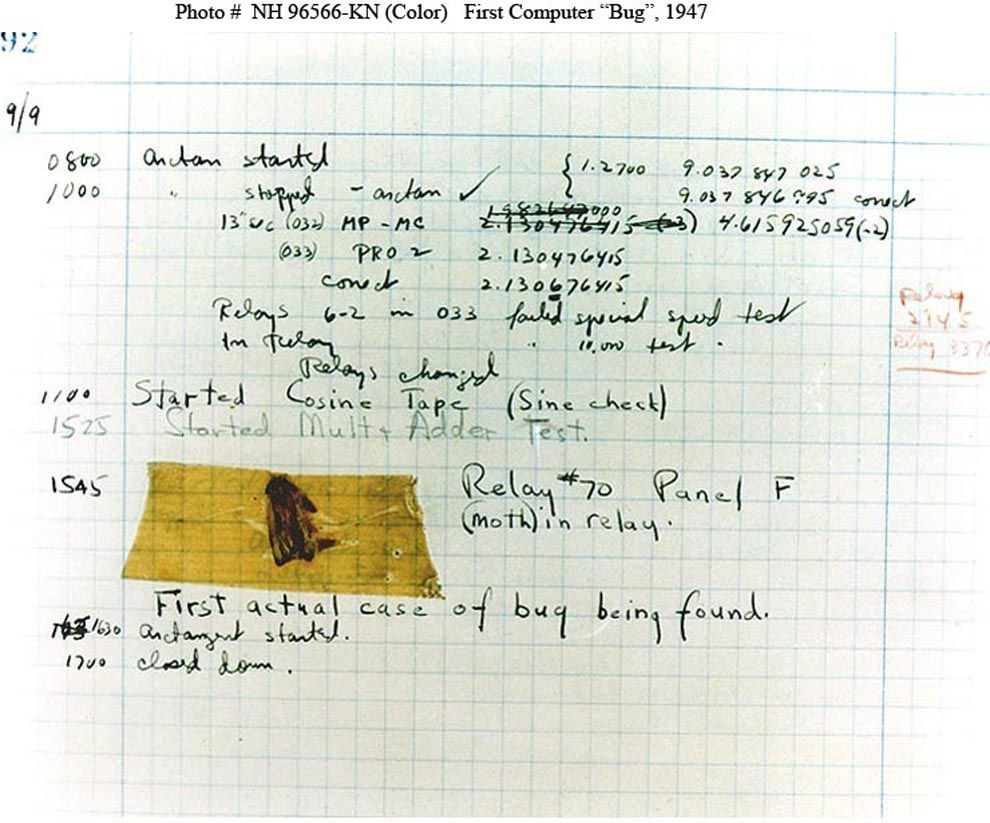
\includegraphics[width=0.4\textwidth]{Figures/first-pc-bug.jpg}
	\caption{Záznam o první počítačové chybě \cite{85SxcMZY6LKfV8v4}}
	\label{fig:WritingThesis}
\end{figure}

\section{Proces vývoje softwaru}
Mezi základní modely popisující proces vývoje softwaru patří model velkého třesku, model „programuj a opravuj“, vodopádový model nebo spirálový model. Mezi stěžení body propracovanějších modelů se řadí specifikace, vývoj a testování.

\subsection{Model velkého třesku}
Metoda vývoje, při kterém se využívá modelu velkého třesku stojí na jednoduchosti celého konceptu. Veškeré úsilí je soustředěno na vývoj softwaru – konečného produktu. Model počítá s velmi nízkou úrovní specifikace produktu. Součástí tohoto modelu není fáze formálního tetování.\cite{Patton2002}


\begin{figure}[h]
	\centering
	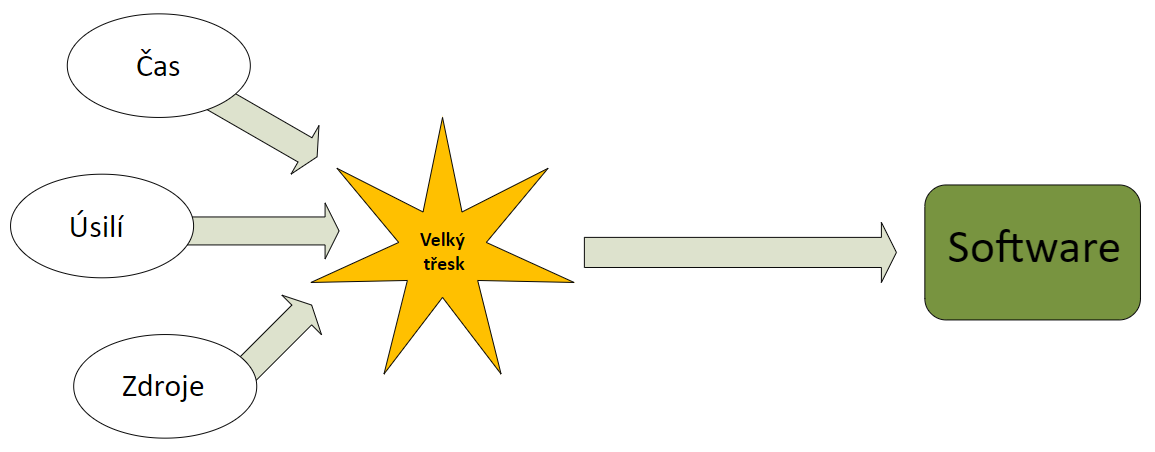
\includegraphics[width=0.8\textwidth]{Figures/velky-tresk.png}
	\caption{Model velkého třesku}
	\label{fig:WritingThesis}
\end{figure}

\subsection{Model „programuj a opravuj“}
Tento model nevyžaduje příliš mnoho režie či řízení. Je určen pro malé projekty vyžadující prezentování výsledků v rychlém sledu. Začíná se hrubou představou o finálním produktu, pokračuje cykly vývoje, testování a opravou chyb. Po několika iteracích těchto cyklů je rozhodnuto o ukončení práce a vydání softwaru. Model „programuj a opravuj“ se v praxi využívá u prototypů.\cite{Patton2002}


\begin{figure}[h]
	\centering
	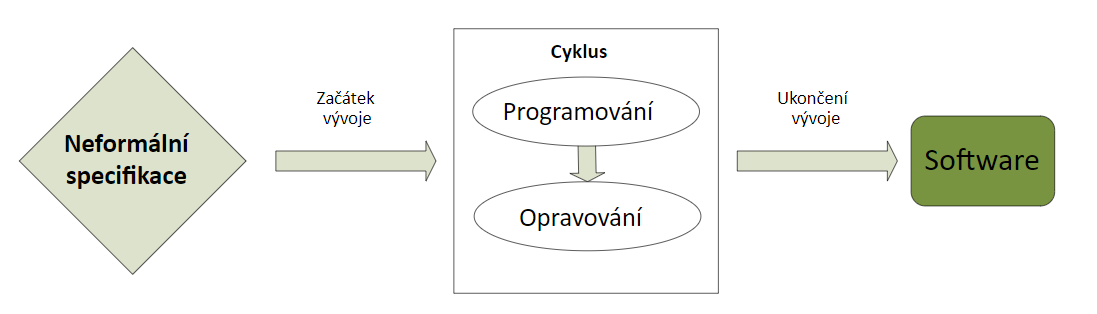
\includegraphics[width=0.8\textwidth]{Figures/programuj-a-opravuj.png}
	\caption{Model „programuj a opravuj“}
	\label{fig:WritingThesis}
\end{figure}

\subsection{Vodopádový model}
Vodopádový model spočívá v kontinuálním vývoji s přesně danou specifikací. Jednotlivé kroky tohoto modelu jsou atomické, nepřekrývají se a „není cesty zpět“. V jednotlivých krocích není možné postupovat zpětně, musí se dokončit daná iterace a začít specifikací znova.\cite{Patton2002}

\begin{figure}[h]
	\centering
	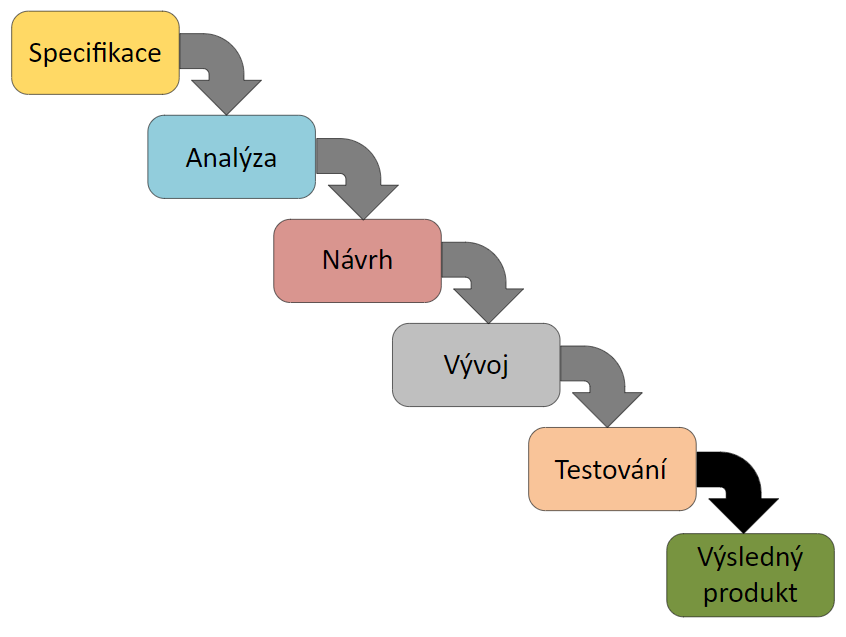
\includegraphics[width=0.5\textwidth]{Figures/vodopad-model.png}
	\caption{Vodopádový model}
	\label{fig:WritingThesis}
\end{figure}

\subsection{Spirálový model}
Spirálový model řeší nedostatky výše uvedených modelů. Vývoj softwaru, který se řídí postupem daným spirálovým modelem je efektivní. Nevýhodou může být podstatně větší režie, než tomu bylo u modelů jako je model velkého třesku či model vodopádový. Jednotlivé kroky ve spirálovém modelu se mohou na rozdíl od vodopádového modelu překrývat.\cite{Patton2002}

V modelu jsou patrné 4 skupiny akcí, které je třeba provádět. Jmenovitě se jedná o plánování, analýzu rizik, vývoj a zhodnocení. Vývoj podle tohoto modelu probíhá v iteracích, při každém průchodu cyklem je pomyslně dokončena další část spirály.



\begin{figure}
	\centering
	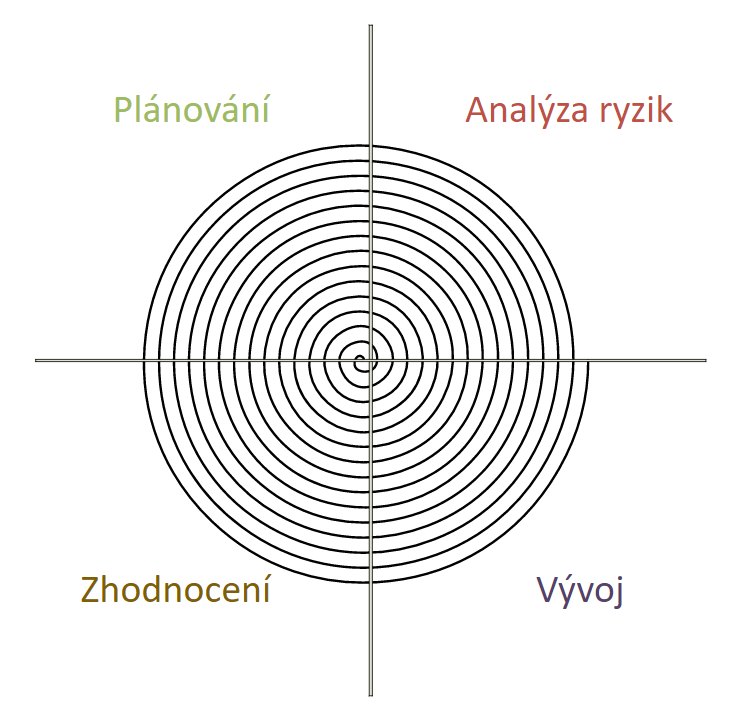
\includegraphics[width=0.6\textwidth]{Figures/spiral-model.png}
	\caption{Zjednodušený spirálový model}
	\label{fig:WritingThesis}
\end{figure}

\begin{figure}
	\centering
	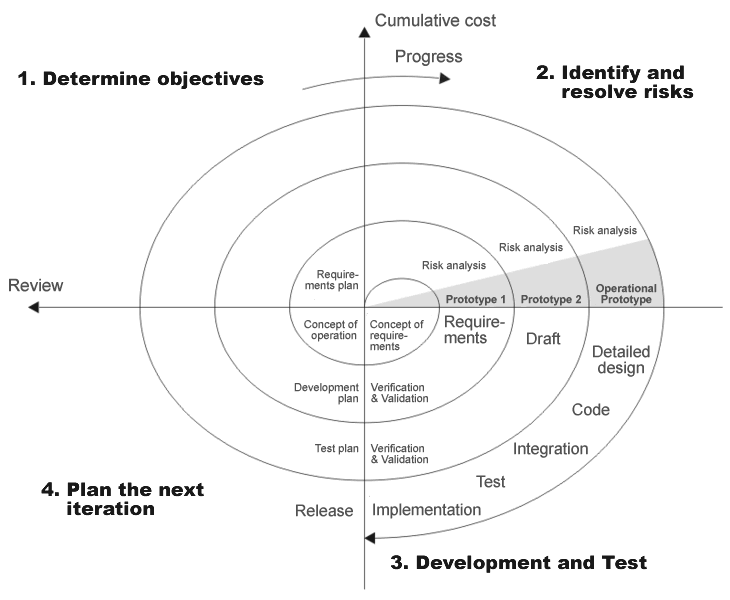
\includegraphics[width=0.6\textwidth]{Figures/Spiral_model_Boehm_1988.png}
	\caption{Spirálový model \cite{ee27bbyhk5LP1Ekm}}
	\label{fig:WritingThesis}
\end{figure}

\section{Manuální a automatizované testování}
Testování softwaru, je možné rozdělit do dvou základních skupin.  Manuální testování zpravidla provádí člověk. Naopak automatizované testování zajišťuje stroj, který dle zvoleného scénáře většinou generuje požadavky na systém a čeká na odpověď, kterou porovnává s předpokládaným výstupem.

Automatizované testování nám může v krátkém čase přinést mnoho zajímavých výsledků, dává nám náhled na to, na co se v daném systému zaměřit. Stojí však na poměrně náročném vytváření testovacích plánů či schémat. V případě nalezení chyby při automatickém testování se ale obvykle k problému musí dostat v posledním kroku i člověk, jehož úkolem je nalezení chyby v kódu. Využití automatizovaných testů je nesporně výhodné, především z časových důvodů, můžeme stejné scénáře spouštět několikrát za sebou, např. s upravenými vstupy, které si můžeme nechat generovat. Výstupem automatizovaného testování je většinou souhrn či stručný přehled akcí, které se provedly. Tyto akce jsou pak označeny, zda se výstup rovná očekávanému výstupu. Automatizované testování se z praktických důvodů přesné specifikace očekávaného výstupu využívá především k testování rozhraní softwaru. V případě projektu HEAppE Middleware jde o testování rozhraní REST API.

\section{Framework pro automatizované testování HEAppE}
Mezi základní úkoly pro automatizované testování softwaru se řadí výběr frameworku . Pro účely HEAppE Middleware byl vybrán Robot Framework \cite{UDdvJfGpGdOGQs2a}. Jedná se o automatizační open-source framework, který pracuje s vytvořenou provozuschopnou aplikací či API. Tento framework\footnote{Framework je set programů, knihoven a rozhraní, které programátorovi zjednodušují práci. Framework většinou stačí nakonfigurovat a používat.} se využívá na úrovni integračního testování, v praxi jde o tzv. smoke testy \cite{K35ZsSqAfq3Ec1XJ}. Hlavním úkolem smoke testů je rychlé vyhodnocení funkčnosti aplikace, aby bylo možné přejít k dalšímu vývoji. Pomáhají odhalit nefunkční části aplikace či aplikačního rozhraní. Robot Framework je schopný pracovat s grafickým uživatelským rozhraním, ale pracuje i na úrovni REST API.

Robot Framework je nezávislý na operačním systému, jádro frameworku stojí na programovacím jazyce Python. To umožňuje především snadnou rozšiřitelnost a použitelnost. Základem automatizovaného testování prostřednictvím Robot Frameworku je sestavení testovacích plánů. Jedná se o popis akcí, které má framework vykonat. V případě HEAppE Midleware bude Robot Framework testovat endpointy REST API, pro dané požadavky budou dynamicky vytvářeny JSON specifikace. Základním plánem pro automatizované testování bude autentizace, vytvoření a spuštění úlohy. Tento plán může být dále rozšiřován.

Velkou výhodou tohoto frameworku je možné napojení na průběžnou integraci ve fázi vývoje. Průběžná integrace (Continuous Integration) slouží k urychlení nalezení chyb, integrace je spouštěna na integračním serveru podle předem zvoleného schématu. Metoda průběžné integrace je využívána i v projektu HEAppE, v průběhu sestavování aplikace je možné provést sadu testů z Robot Frameworku. Vývojáři pak budou mít lepší přehled o funkčnosti systému v dané fázi vývoje. Průběžná integrace je spouštěna předem nastavenou akcí, může se jednat například o úpravu repozitáře\footnote{Repozitář je typ datové úložiště verzovacího systému.}  či dané větve repozitáře projektu. Sestavení a smoke testy jsou pak spouštěny automaticky, vývojář tak může sledovat stav integrace s informacemi o provedených testech. 

\begin{figure}[h]
	\centering
	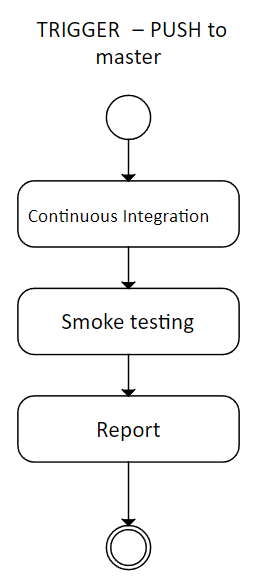
\includegraphics[width=0.2\textwidth]{Figures/cont-integration-diagram.png}
	\caption{Průběžná integrace a smoke testování}
	\label{fig:WritingThesis}
\end{figure}

\section{Testovací scénář pro HEAppE}
Robot Framework je skvělým kandidátem pro testování hotových softwarových řešení. Pomocí tohoto frameworku je možné otestovat aplikační rozhraní daného systému z pohledu uživatele. Pro komplexní otestování HEAppE je možné vytvořit několik testovacích scénářů, které na sebe mohou navazovat. Základním scénářem pro používání HEAppE Middleware je vytvoření a spuštění úlohy na výpočetním clusteru. Z tohoto případu užití vychází i základní scénář pro automatizované testování HEAppE prostřednictvím Robot Framework.

Důležitým krokem při užívaní HEAppE Middleware je provedení autentizace. HEAppE po úspěšné autentizaci uživatele vrátí vygenerovaný unikátní identifikátor, který uživatel následně přidává do každého dalšího příkazu.

Hlavním úkolem tohoto testovacího plánu bude otestování spouštění úloh na dvou výpočetních clusterech. Na každý cluster bude podána žádost o spuštění tří konfigurací úloh (jednoduchá, s generickým command templatem a extra dlouhá úloha).

Před spouštěním úloh budou otestovány funkcionality související s uživatelem HEAppE. Tyto kroky se nachází v následující tabulce.

\newcommand{\specialcell}[2][c]{%
  \begin{tabular}[#1]{@{}c@{}}#2\end{tabular}}

\begin{table}
	\centering
	\label{tab:TopLevelTableLabel}
		\begin{tabular}{|c|c|c|}
		    \hline
		    Krok & Název & Endpoint \\
		    \hline
			1 & Získání seznamu dostupných clusterů & \specialcell{/heappe/ClusterInformation/\\ListAvailableClusters}\\
			\hline
			2 & Autentizace uživatele & \specialcell{/heappe/UserAndLimitationManagement/\\
			AuthenticateUserPassword}\\
            \hline
			3 & \specialcell{Získání využití zdrojů a limity\\ uživatele HEAppE} & \specialcell{/heappe/\\UserAndLimitationManagement/\\GetCurrentUsageAndLimitationsForCurrentUser}\\
            \hline
            4 & \specialcell{Získání využití zdrojů na výpočetních \\clusterech} & 	\specialcell{/heappe/ClusterInformation/\\CurrentClusterNodeUsage}\\
            \hline
            5 & Získání využití zdrojů uživatele HEAppE & \specialcell{/heappe/JobReporting/\\GetUserResourceUsageReport}\\
            \hline
            6 & \specialcell{Získání využití zdrojů skupiny uživatelů\\HEAppE} & \specialcell{/heappe/JobReporting/\\GetUserGroupResourceUsageReport}\\
            \hline
		\end{tabular}
	\caption{Seznam kroků pro testování funkcionalit související s uživatelem HEAppE}
\end{table}

**TABULKA

Krok	Název	Endpoint
1	Vytvoření úlohy	/heappe/JobManagement/CreateJob
2	Spustit zpracování úlohy	/heappe/JobManagement/SubmitJob
3	Získání spotřebovaných zdrojů úlohy	/heappe/JobReporting/GetResourceUsageReportForJob
4	Získání využití zdrojů na výpočetních clusterech	/heappe/ClusterInformation/CurrentClusterNodeUsage
5	Získání stavu úlohy	/heappe/JobManagement/GetCurrentInfoForJob
6	Vyčkání na spuštění úlohy	/heappe/JobManagement/GetCurrentInfoForJob
7	Získání IP adres alokovaných uzlů	/heappe/JobManagement/GetAllocatedNodesIPs
8	Zrušení úlohy	/heappe/JobManagement/CancelJob
9	Vyčkání na ukončení úlohy	/heappe/JobManagement/GetCurrentInfoForJob
10	Smazání úlohy	/heappe/JobManagement/DeleteJob



Dále bude otestováno spouštění třech různých úloh na dvou různých superpočítačových clusterech. Kroky určené k otestování jedné úlohy popisují kroky uvedené v následující tabulce.


Protože je práce s úlohou na výpočetním clusteru řízena plánovačem, prakticky se jedná o předávání pokynů. Proto se v testovacím plánu musí vyskytovat čekání na vykonání příkazu. Při pokynu pro spuštění úlohy tak musíme čekat na to, až naši úlohu spustí plánovač na výpočetním clusteru. V testovacím scénáři je toto čekání implementováno cyklickým doptáváním HEAppE REST API s prodlevou, aby nedošlo k zablokování (toto chování by mohlo nést znaky DOS/DDOS útoku\footnote{DDOS nebo také DOS je typ útoku na internetové služby nebo stránky, jehož cílem je cílovou službu znefunkčnit a znepřístupnit ostatním uživatelům; může k tomu dojít zahlcením obrovským množstvím požadavků, ve variatně DDOS jde o distribuovaný DOS\cite{UUBpn6UTaV8mOipc}}). Následuje ukázka kódu testovacího scénáře Robot Frameworku obsahujícího popsané cyklické doptávání REST API. V tomto případě se cyklus se ukončí, pokud HEAppE vrátí stav, který značí, že je úloha spuštěna. Očekává se, že se stav změní v rámci jednotek či desítek minut, Roboto Framework neumožňuje práci s cykly s neznámým počtem opakování, proto byl při implementaci využit cyklus se známým počtem opakování.

Útržek testovacího scénáře obsahuje funkci WaitForJobRuns, úkolem této metody je počkat na spuštění úlohy plánovačem na výpočetním clusteru.

\newpage
\lstinputlisting[language=bash, caption={Segment Robot Framework testu}]{SourceCodes/wait-for-job-runs.txt}

Výsledkem tohoto testování je vygenerovaný report, programátor má pak lepší představu o funkčnosti jednotlivých částí systému. Tyto reporty Robot Framework připraví v grafické podobě, dostupné jsou ve formátu html. Surová data jsou součástí reportu ve struktuře XML\footnote{Výměnný formát pro přenos dat}.



\begin{figure}[h]
	\centering
	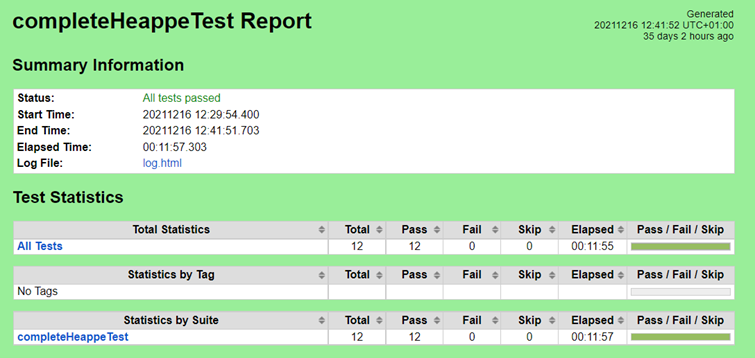
\includegraphics[width=0.95\textwidth]{Figures/report-small.png}
	\caption{Report Robot Frameworku}
	\label{fig:WritingThesis}
\end{figure}

Z výše uvedeného reportu můžeme vyčíst, že provedení scénáře trvalo pod 12 minut, pokud by tento scénář měl replikovat člověk, trvalo by to minimálně dvojnásobně déle. Tento test je prováděn pravidelně a několikrát za sebou, počáteční časové náklady na sestavení tohoto scénáře jsou nesrovnatelné s přínosem. Test navíc může běžet v pozadí automaticky a vývojář si tak jen vyzvedne výsledek. Následuje část reportu, který obsahuje i podobnější informace o každém provedeném kroku.


Tento testovací scénář je možné volně rozšiřovat nebo vytvářet scénáře obdobné. Velmi praktické je i využití Robot Frameworku pro testování softwaru v době vývoje. Scénář můžeme měnit podle aktuálních požadavků např. při vývoji nové funkcionality.

